\documentclass[11pt]{article} % use larger type; default would be 10pt
\usepackage[utf8]{inputenc} % set input encoding (not needed with XeLaTeX)

%%% BEGIN Article customizations

%%% PAGE LAYOUT
\usepackage{geometry} % to change the page dimensions
\geometry{a4paper} % or letterpaper (US) or a5paper or....
% \geometry{margin=1in} % for example, change the margins to 2 inches all round
\usepackage[parfill]{parskip} % Activate to begin paragraphs with an empty line rather than an indent

%%% FIGURES
\usepackage{graphicx} % support the \includegraphics command and options
\graphicspath{{../FIGURES/FIGURE_PDFS/}}

%%% PACKAGES
\usepackage{booktabs} % for much better looking tables
\usepackage{array} % for better arrays (eg matrices) in maths
\usepackage{paralist} % very flexible & customisable lists (eg. enumerate/itemize, etc.)
\usepackage{verbatim} % adds environment for commenting out blocks of text & for better verbatim
\usepackage{subfig} % make it possible to include more than one captioned figure/table in a single float
% These packages are all incorporated in the memoir class to one degree or another...

%%% HEADERS & FOOTERS
\usepackage{fancyhdr} % This should be set AFTER setting up the page geometry
\pagestyle{fancy} % options: empty , plain , fancy
\renewcommand{\headrulewidth}{0pt} % customise the layout...
\lhead{}\chead{}\rhead{}
\lfoot{}\cfoot{\thepage}\rfoot{}

%%% SECTION TITLE APPEARANCE
\usepackage{sectsty}
\allsectionsfont{\sffamily\mdseries\upshape} % (See the fntguide.pdf for font help)
% (This matches ConTeXt defaults)

%%% ToC (table of contents) APPEARANCE
\usepackage[nottoc,notlof,notlot]{tocbibind} % Put the bibliography in the ToC
\usepackage[titles,subfigure]{tocloft} % Alter the style of the Table of Contents
\renewcommand{\cftsecfont}{\rmfamily\mdseries\upshape}
\renewcommand{\cftsecpagefont}{\rmfamily\mdseries\upshape} % No bold!

%%% END Article customizations

%%% The "real" document content comes below...

\title{Double Sequencing Analysis (this still needs a title)}
\author{Dakota Z. Derryberry, Claus O. Wilke, Matthew C. Cowperthwaite}

\begin{document}
\maketitle

\section{Introduction}

Intro goes here.

\section{Results}

\subsection{Unfiltered data: WGA v. WGS}

As expected, we found that 

% \begin{figure}
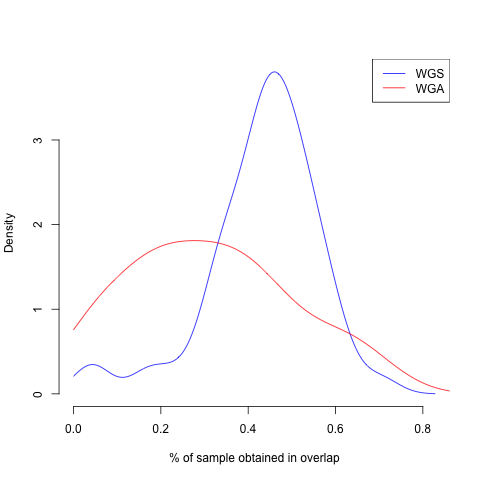
\includegraphics[scale=0.5]{unfiltered_overlap_WGS_WGA_together_densities.png}
% \end{figure}

\subsection{Unfiltered data: Time points}

\subsection{Filtering}

\section{Methods}

\subsection{Data and back-end processing}

All sequence data came from The Cancer Genome Atlas (TCGA) Gliobastoma multiforme (GBM) data set. We downloaded raw reads in (XXX format) using (CGHub?) on (date) for 68 patients. For each patient, data consisted of one set of rads taken from blood DNA, and two sets of reads taken from tumor DNA. In 55 cases, the two sets of reads from tumor DNA were one set of reads from whole genome sequencing (WGS) and one set of reads from whole genome sequencing with amplification (WGA). In 13 cases, the two sets of reads from tumor DNA were one set of reads pre-readiation treatment and one set post-radiation treatment. We developed a pipeline to align all reads to HG19. This pipeline used (bowtie?) for alignment and (bedtools? whatever -- quality control...) We used SomaticSniper to align each tumor sequence with it's corresponding blood sequence. We then filtered the SomaticSniper data using 8 custom filters. These removed (i) , (ii) , (iii) , (iv) , (v) , (vi) , (vii) , and (viii) . All custom code is available in a github repository, located at (webaddress). In addition to sequence data, filter 6 uses dbSNP, version 137, to find common SNPs among the putative mutaitons called by SomaticSniper.

\subsection{Analysis}

We used custom python scrips, available in the above github repository, to perform simple calculations and data operations. We used R to do statistics and generate figures, and this code is also availabel in the git repository.  

\section{Discussion}

What do I think of this?

\end{document}
